\chapter{Introduction}
	\label{chapter:Introduction}
	\section{About this document}
	
"Soundgates – Interactive Music Synthesis on FPGAs" is a project initiated by the Computer Engineering Group of the University of Paderborn, aiming to synthesize music on modern FPGAs. 
Furthermore, users should be able to interact with the system in a playful way by manipulating the synthesized music with advanced sensors such as the acceleration sensor in modern smartphones or motion capturing techniques like Kinect.


This document is the project plan of our project group.
Not only should this document serve as a basis for the later evaluation and grading, 
but also as a reference for our group during the main working phase running from \todo{??.2013 to ??.2014.}

This first chapter introduces concepts and system that we plan to use to achieve the goals outlined in Chapter \ref{chapter:Goals}. 
Chapter \ref{chapter:RelatedWork} mentions existing systems similar to what we are going to create.
Finally Chapters \ref{chapter:Organization} and \ref{chapter:Workplan} describe how the group will organize itself and the groups' milestones.

	\section{Definitions}
	 The following table displays some definitions, that will be used throughout this document.
	\todo{LF: Tabelle erstellen/vervollständigen!!}
	 %\begin{tabular}[h]{|c|p{9.75cm}|}
	 % \hline
	 % Term & Definition \\
	 % \hline
	 % \hline
	 % Composite Component & Definition \\\hline
	 % Component & A basic building block to generate music ??Haben wir uns hier auf Block als Bezeichnung geeinight? Component eher im Sinne von Softwarekomponente\\\hline
	 % Editor & The Editor is used to create a patch out of components to generate synthesizable code which can be put on a FPGA \\\hline
	 % FPGA & Field Programmable Gate Array \\\hline
	 % Patch & The entire system which consists of Components and Composite Components. A set of single Components can build a new Component \\\hline
	 % Port & The interface from one Component to another one \\\hline
	 % Simulation & The developed patch is played through the PC speakers \\\hline
	 %\end{tabular}
	 
	 % Usage of the acronym-package:
	 % !!Usually reference with \ac{FPGA} (prints at the first usage the long form along with the short from and on of all the following uses only the short form will be printed)
	 % \acs{FPGA} (short only), \acf{FPGA} (short and long), \acl{FPGA} (long only)
	%\todo{Von den Elementen in dieser Liste ist das meiste gar kein Akronym (und wird ohne Benutzung im Text entsprechend auch nicht angezeigt)}
	 %\begin{acronym}[Soundgates]
	  %\acro{ADSR}{Attack, Decay, Sustain, Release}
	  %\acro{Component}{A basic building block to generate music \todo{??Haben wir uns hier auf Block als Bezeichnung geeinight? Component eher im Sinne von Softwarekomponente}}
	  %\acro{Editor}{The Editor is used to create a patch out of components to generate synthesizable code which can be put on a FPGA}
		%\acro{DAC}{Digital Analog Converter}
	  %\acro{FPGA}{Field Programmable Gate Array}
	  %\acro{Patch}{The entire system which consists of Components and Composite Components. A set of single Components can build a new Component}
	  %\acro{Port}{The interface from one Component to another one}
	  %\acro{Simulation}{The developed patch is played through the PC speakers}
	 %\end{acronym}
	 

	\section{Generative music}
	

	\subsection{Introduction}
	\todo{Kaputte Zitate}
	As pointed out in \cite{Chandra2012}, there are many cultures where musicical experience is defined by people performing and people perceiving music. 
	The only way to slightly exert influence on the performer's music is by cheering, shouting, etc. on a concert. 
	
	The gap between performer and perceiver reaches its peak in the context of recorded music like CDs or MP3 files as the listener cannot manipulate the music in any way. 
	However, there is a rising trend for musical interaction either on your own or in a social group, like in the video game "Guitar Hero" \cite{Chandra2012, Planck2009}. 
	Even without any musical knowledges or talent, it is more and more possible to interact, manipulate or even create music.
	Generative music combines the opportunities of making music without having knowledges of how to play an instrument and explicitly exert influence on music you hear.
	An early and popular example of generative music was Mozart's musical dice game. Given a set of small sections of music, it was randomly chosen which part was played next.


	\subsection{Approaches} 

	Generative music (or algorithmic music) can be divided into the following subcategories \cite{Wooller2005}.

	\subsubsection{Linguistic/Structural}

	Already existing songs are initially scanned and afterwards recomposed randomly. 
	The technique is to create a grammar from the original song. The production rules of this grammar are derived from subsequent pairs of notes. By executing a random, applicable rule a new song is generated.

	\subsubsection{Creative/Procedural}

	Mozart's dice game, already mentioned in the introduction, falls into this category.
	There are different processes/procedures which play predefined music. These processes have an arbitrary order and starting time. 

	\subsubsection{Biological Emergent}

	Music is generated by biological or natural phenomenons, i.\,e. by differing parameters within an ecology, for example wind-chimes. Element of the chime are able to play specific sounds. Which sounds are played emerges from the blowing wind.

	\subsubsection{Interactive/Behavioural}

	The interactive/behavioural generative music approach results from processes without discernable musical inputs. It is a question of synthesized music and recorded and filtered samples at the most. The music generation is fully controlled by user input and interaction. 
	The easiest examples are digital synthesizers, such as Ableton or Cycling '74 Max. There are no instrumental musical inputs. Instead, the music is generated by synthesizing waveforms and by combining and filtering them. Furthermore it is possible to take influence on this music, by modifying inputs like frequencies and so on. Most of this interaction still needs some musical knowledge, but there are also approaches that allows the user to simply modify the music by using acceleration sensors in modern smartphones.
	
	This is the initial point on what this project is based: synthesizing music along with a highly interactive interface to exert influence on the music.

	\section{Possible User Interactions}
	In order to make the system interactive there need to be one or more interfaces, over which the user can take influence on the music. This could happen via a midi keyboard or other electronic instruments. But with the purpose of providing an easy, playful access to music generation without knowledges of an instrument, we are focussing on advanced sensors. Sensors like Microsoft's Kinect systems can easily track e.\,g. the user's hand. An intuitive way of changing system's parameters is to measure and transmit the height of the hand. Other possible sensors can be found in nearly every modern smartphone, e.\,g. the acceleration sensors.
	
			
				
	\section{Introduction to sound synthesis}
		Sound synthesis is the artificial creation of sound. 
		Cleverly built synthesizers can mimic many real instruments 
		and of course are also able to create sounds with no real world counterpart.
		
		The first synthesizers consisted of seperate analog building blocks.
		A user could connect these blocks with cables in many different ways to generate, modify and filter a signal, depending on the order and fashion of the blocks.
		As with many other systems digital components replaced the analog ones over time.
		The general approach, however, remained the same. 
		Users do not necessarily plug in cables anymore but conceptually one still connects separate building blocks to create the sound that he wants.
		
		The most basic digital synthesizer would be the one shown in Figure \ref{fig:sound_generation}. 
		In this example an oscillator generates a waveform, for example a basic sine wave.
		Sampled values of the waveform are fed into an \ac{DAC} which converts them to an analog signal which can then be played on a speaker.
		While it is not very pleasing to listen to an unmodified sine wave, it is already some artifical and therefore synthesized sound.
		
	  	\begin{figure}[!h]
		\centering
			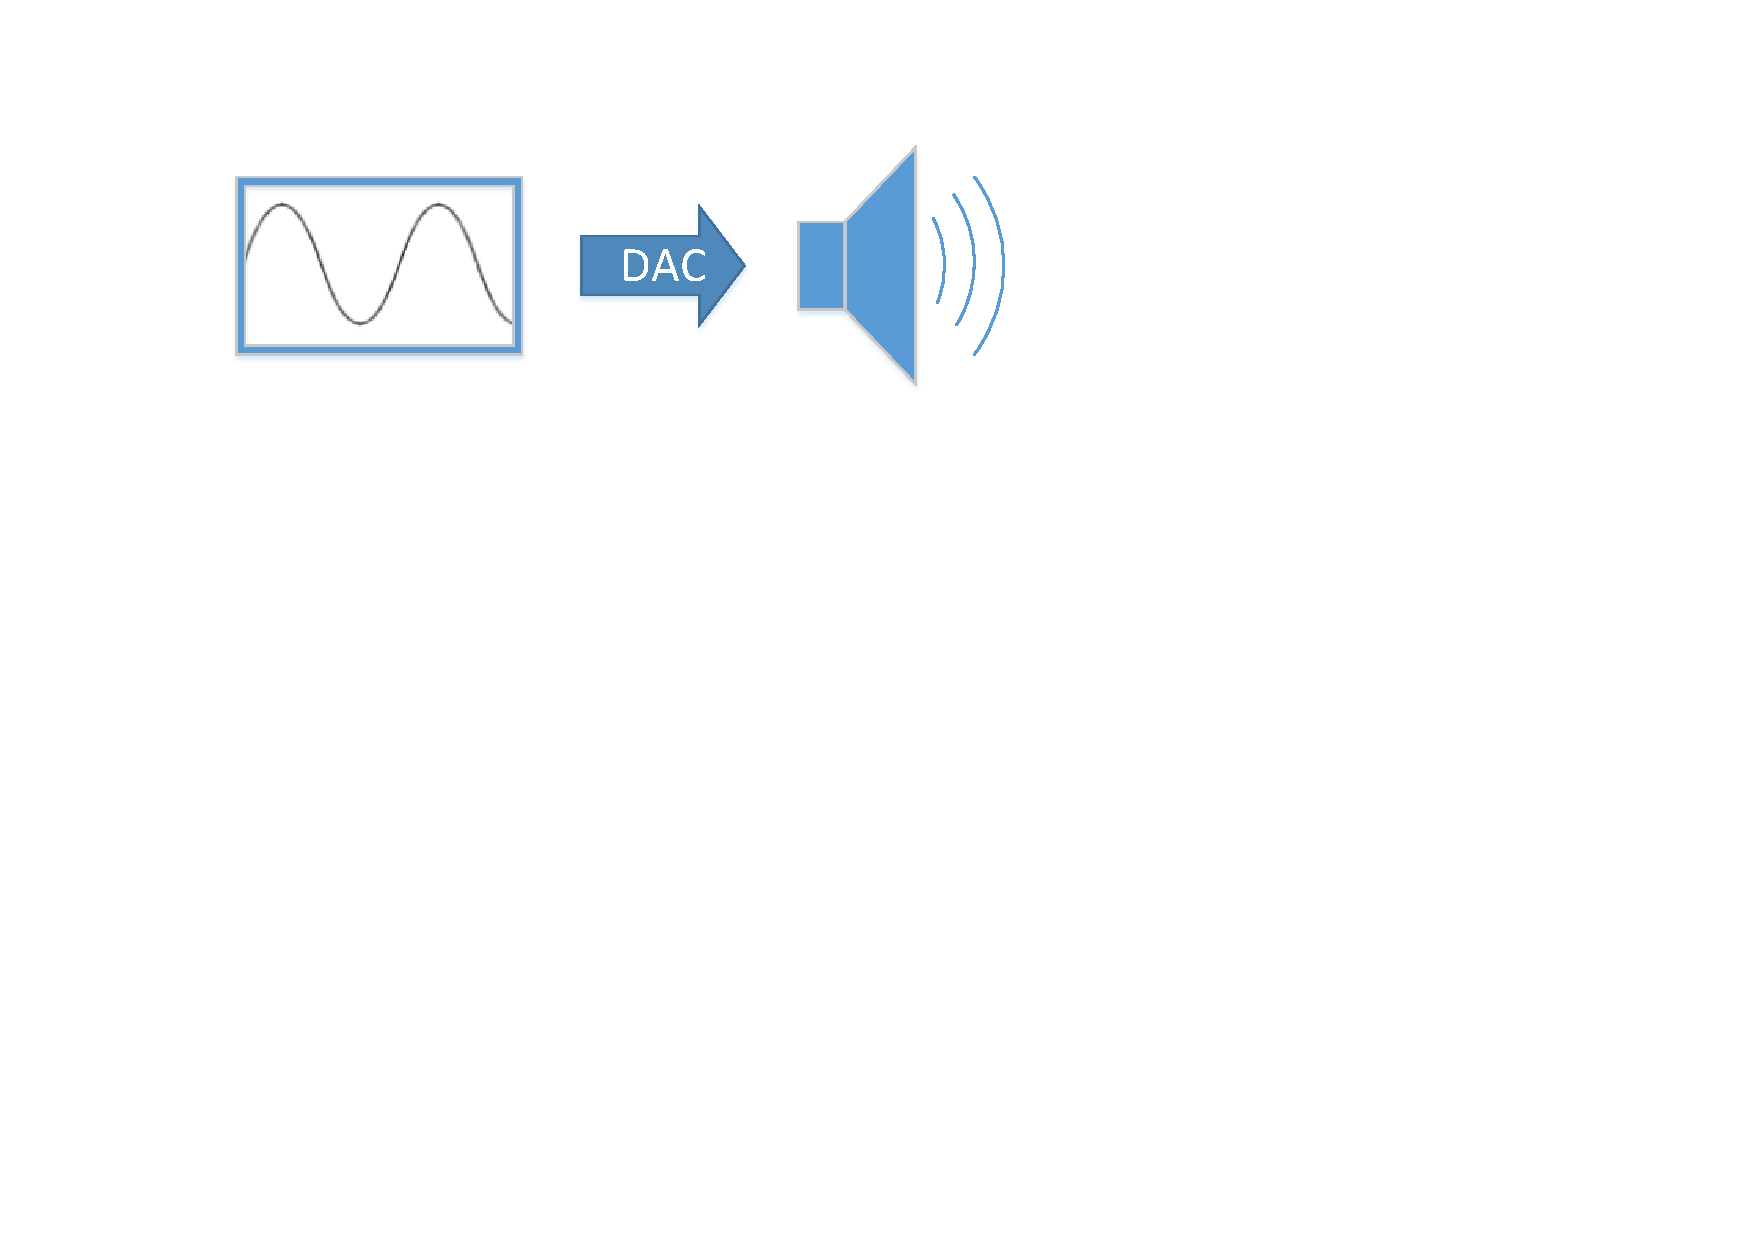
\includegraphics[width=0.90\textwidth]{images/sound_generation.pdf}
		\caption{Easiest way to generate sound on a digital system }
		\label{fig:sound_generation}
		\end{figure}
		
		\subsection{Frequency and notes}
		The previous example only used a single sine wave. 
		With a small addition this setup can already be used to play notes.
		The only thing that needs to be added would be a way to control the frequency of the sine wave since the value of a note is determined only by the frequency of the sound wave. 
		440 Hz for example corresponds exactly to an A4.
		This is true regardless of the actual shape of the waveform, be it a sine wave, a square wave or something completely different. 

		Thinking of different instruments this circumstance quickly becomes obvious. 
		While both a violin and a piano can play the same specific note, it will sound differently on both instruments.
		This difference is due to the fact, that the sound waves those instruments create have a different shape.
		This characteristic of a sound is called \emph{timbre} or \emph{sound color}.
		
		\subsection{Waveform generation}
		Creating a specific base shape of our waveform can be done in several ways, each with it's advantages and disadvantages and a spectrum of sounds that can be created.
		Of course, many of these approaches are not mutually exclusive but can be combined with each other.
			\subsubsection{Additive synthesis}
				In additive synthesis a sound designer uses multiple basic waveforms with different frequencies, usually sine waves, adds up their outputs and normalizes the result.
				For example, adding a sine wave with frequency $2F$ to a sine wave with frequency $F$ would result in a different sound color but still with an overall frequency of $F$ and therefore the same note.
				
				The sound designer has very tight control over the produced sound with additive synthesis.
				According to the fourier theorem it is possible to approximate every periodic function by the combination of sines. 
				Therefore, a real world sound could be analyzed and rebuilt this way.
				However this approach may need a lot of separate oscillators and might therefore become unfeasible to handle for very complex sounds with a broad frequency spectrum.
			\subsubsection{Subtractive synthesis}
				Subtractive synthesis starts with waveforms like a sawtooth, square, triangle or even periodic noise.
				Contrary to a bare sine wave, these patterns have already a wide frequency spectrum. 
				By feeding these waves into different filters (section \ref{subsec:filters}) this broad spectrum can then be reduced again. 
				
				Compared to additive synthesis, it is cheaper to create rich sounds with subtractive synthesis but it sacrifices the very tight control over every single frequency.
			\subsubsection{Frequency/amplitude modulation}
				Another possibility is to modify the frequency or amplitude of one waveform by the value of another.
				This can create relatively rich results with relatively little effort.
				However, this approach usually creates hearable vibrato or tremolo effects which only fit for specific desires.
			\subsubsection{Pre recorded samples}
				Any result of the aforementioned approaches as well as real sound can of course be saved and reused.
				It is relatively cheap and efficient to store small sound samples. 
				Instead of calculating the values of a sine wave, they could just be taken from a lookup table.
				Or instead of trying to synthesize a violin, a real one could be recorded and sampled later for further use.
				
				Such samples are very inflexibile of course.
				It is possible to modify the frequency within limits and it is possible to	process the samples further, but they cannot serve as the only basis for a synthesizer that should be able to create arbitrary sound.			
		\subsection{Further transformation}

			A cleverly designed waveform that was created with any of the previous approaches might already sound more or less pleasing but still is rather monotonous on its own.
			
			\subsubsection{Filters} 
				\label{subsec:filters}
				Filters were already mentioned in the subtractive synthesis section. 
				These are components that are able to modify a signal depending on its frequency.
				
				There exist filters to either apply to high or low frequencies or to specific bands of frequencies.
				Frequencies outside their scopes can pass almost unhindered while all others are attenuated or completely suppressed.
			\subsubsection{Envelope modulation}
				Real instruments have varying loudness values while playing a single note.
				A common shape would be	\ac{ADSR}.
				In the first phase, the note is not already played at maximum volume but raises in a step curve towards it.
				It falls to a medium level in the decay phase which is held during the sustain phase.
				The sustain phase ends once the key (eg. on a piano) is released and then the sound fades out in the decay phase.
				
				This pattern can be used for many instruments, especially pianos exhibit a default \ac{ADSR} pattern. An exemplary \ac{ADSR} pattern is shown in figure \ref{fig:adsr}
				Other instruments might skip some of the phases. 
				Of course, for the creation of artificial sounds, one can also think of additional phases.
				
				\begin{figure}[!h]
				\centering
					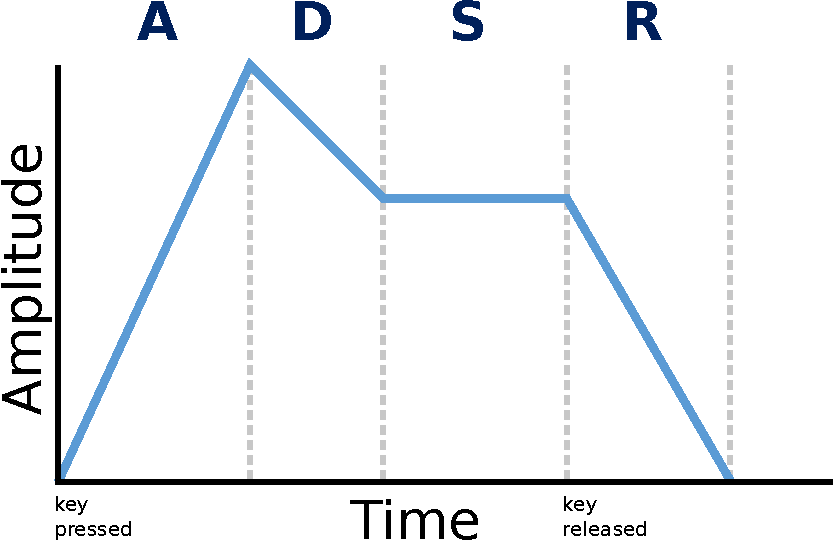
\includegraphics[width=0.70\textwidth]{images/adsr.pdf}
				\caption{\ac{ADSR} envelope}
				\label{fig:adsr}
				\end{figure}
				
			\subsubsection{Other elements}
				There exist some more elements that exceed the pure sound synthesis, but are important for music production and will also be covered by our system.
				For example to create effects like echos, reverberations or chorus the original sound needs to played again with some delay.
			
				Acceleration and Decceleration of a sound signal can be achieved by resampling the original sound with a different rate. This however also changes the pitch.
				But there also exist pitch shifter or time stretchers to change either of the two without affecting the other.
		
		
		
		%- Artifical generation of sound
	  %- Generation of basic waveforms
	    %- More complex and rich patterns by methods like additive/subtractive/... synth 
	  %- Further addition of filters etc
	  %
	  %- Originated from analog synthesizers, nowadays mostly digital. Software for general purpose PCs exist
	  %
	  %- Building patches: job of a sound designer, rather than a musician
			
			
			
			%\section{Project outline}  -- das steht in goals oder?
	  %- Creating an editor for synthesizers. 
	  %- Components of the synthesizer implemented in hardware (and software for simulation purpose)
	  %- Implementation of generative music concepts
	  %------- Warum wollen wir das eigentlich tun? Was ist die Motivation dahinter (zumal es das aus Oslo ja aschon in Software gibt)
		
	\section{Employed systems}
	  \subsection{Xilinx Platform Studio}
	    The overall hardware system is implemented in VHDL, using the Xilinx Platform Studio (XPS), which offers the MicroBlaze Softcore Processor. Additionally it provides the possibility to synthesise the source code.
	  
	  \subsection{ReconOS}
		ReconOS is an Operating System which can be run on a softcore CPU on a FPGA. Through it's support for the Linux kernel it is possible to write applications which consist of Hard- and Software threads. Software threads can be written in C, whereas Hardware threads have to be described in VHDL. The communication between these threads is abstracted through simple function calls. Therefore it is easy to extend an application by calculating time consuming algorithms in hardware, whereas the program flow is controlled in software.

	  \subsection{Eclipse/GMF}
		We avoid building a new graphical editor from ground up since this is an error prone process. Instead we rely on the Model Driven Software Development process for graphical editors which is provided by the GMF framework. Therefore we can generate an editor by specifying the Meta-Model. The graphical surface with our components and connections are the result. Additionally it is necessary to provide functions for every component, so it will be possible to simulate the generated output.      